% BlinkTwin architecture. Build: pdflatex architecture.tex && pdfcrop --margins 4 architecture.pdf ../architecture.pdf
\documentclass{article}
\usepackage[paperwidth=24cm,paperheight=14cm,margin=0pt]{geometry}
\usepackage[T1]{fontenc}
\usepackage{lmodern}
\usepackage{tikz}
\usetikzlibrary{positioning,arrows.meta,fit,backgrounds}
\pagestyle{empty}
\begin{document}
\noindent
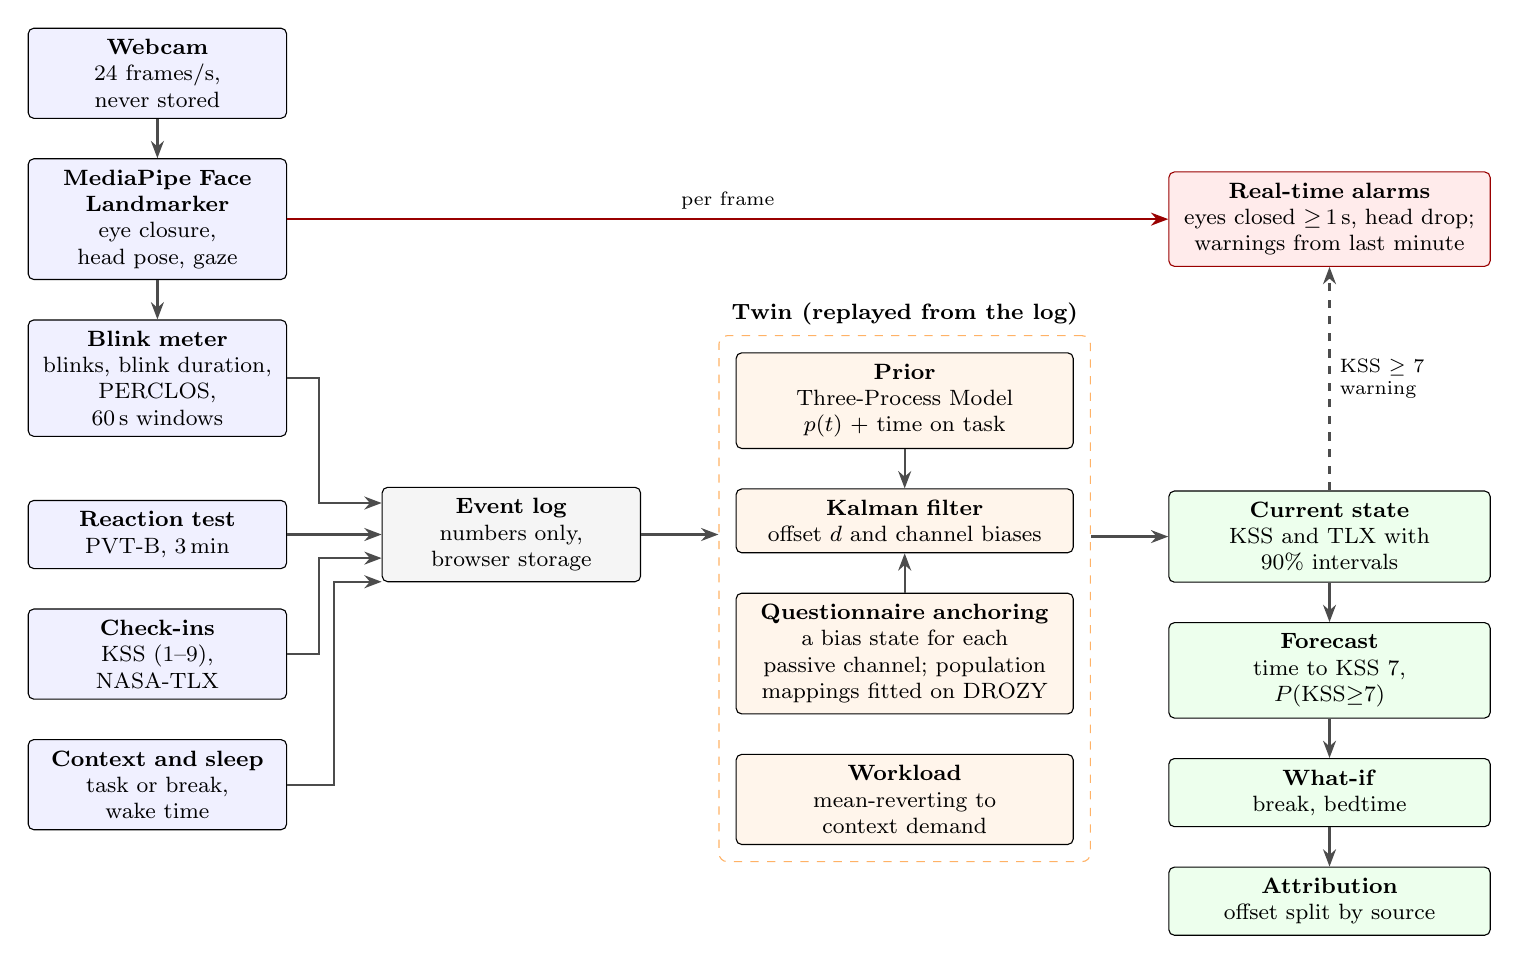
\begin{tikzpicture}[
  font=\footnotesize,
  node distance=5mm and 9mm,
  box/.style={draw, rounded corners=2pt, align=center, inner sep=4pt, text width=#1, fill=white},
  box/.default=30mm,
  srcbox/.style={box=30mm, fill=blue!6},
  corebox/.style={box=40mm, fill=orange!8},
  outbox/.style={box=38mm, fill=green!7},
  alarmbox/.style={box=38mm, fill=red!8, draw=red!60!black},
  arr/.style={-{Stealth[length=2.2mm]}, thick, draw=black!70},
]
% inputs (left column)
\node[srcbox] (cam) {\textbf{Webcam}\\ 24 frames/s, never stored};
\node[srcbox, below=of cam] (mp) {\textbf{MediaPipe Face Landmarker}\\ eye closure, head pose, gaze};
\node[srcbox, below=of mp] (bm) {\textbf{Blink meter}\\ blinks, blink duration,\\ PERCLOS, 60\,s windows};
\node[srcbox, below=8mm of bm] (pvt) {\textbf{Reaction test}\\ PVT-B, 3\,min};
\node[srcbox, below=of pvt] (q) {\textbf{Check-ins}\\ KSS (1--9), NASA-TLX};
\node[srcbox, below=of q] (ctx) {\textbf{Context and sleep}\\ task or break, wake time};

% event log
\node[box=30mm, fill=black!4, right=12mm of pvt] (log) {\textbf{Event log}\\ numbers only,\\ browser storage};

% twin core
\node[corebox, right=12mm of log, yshift=17mm] (tpm) {\textbf{Prior}\\ Three-Process Model\\ $p(t)$ + time on task};
\node[corebox, below=of tpm] (kf) {\textbf{Kalman filter}\\ offset $d$ and channel biases};
\node[corebox, below=of kf] (blr) {\textbf{Questionnaire anchoring}\\ a bias state for each\\ passive channel; population\\ mappings fitted on DROZY};
\node[corebox, below=of blr] (ou) {\textbf{Workload}\\ mean-reverting to\\ context demand};
\begin{scope}[on background layer]
  \node[draw=orange!60, dashed, rounded corners=3pt, inner sep=6pt, fit=(tpm)(ou), label={[font=\footnotesize\bfseries]above:Twin (replayed from the log)}] (twin) {};
\end{scope}

% outputs
\node[outbox, right=12mm of kf, yshift=-2mm] (now) {\textbf{Current state}\\ KSS and TLX with\\ 90\% intervals};
\node[outbox, below=of now] (fc) {\textbf{Forecast}\\ time to KSS 7,\\ $P(\mathrm{KSS}{\geq}7)$};
\node[outbox, below=of fc] (wi) {\textbf{What-if}\\ break, bedtime};
\node[outbox, below=of wi] (why) {\textbf{Attribution}\\ offset split by source};

% arrows
\draw[arr] (cam) -- (mp);
\draw[arr] (mp) -- (bm);
\draw[arr] (bm.east) -- ++(4mm,0) |- ([yshift=4mm]log.west);
\draw[arr] (pvt) -- (log);
\draw[arr] (q.east) -- ++(4mm,0) |- ([yshift=-3mm]log.west);
\draw[arr] (ctx.east) -- ++(6mm,0) |- ([yshift=-6mm]log.west);
\draw[arr] (log.east) -- (twin.west |- log.east);
\draw[arr] (tpm) -- (kf);
\draw[arr] (blr) -- (kf);
\draw[arr] (twin.east |- now.west) -- (now.west);
\draw[arr] (now) -- (fc);
\draw[arr] (fc) -- (wi);
\draw[arr] (wi) -- (why);
% real-time alarm path (per frame, independent of the twin's minute-level state)
\node[alarmbox] at (mp -| now) (alarm) {\textbf{Real-time alarms}\\ eyes closed $\geq$\,1\,s, head drop;\\ warnings from last minute};
\draw[arr, draw=red!60!black] (mp.east) -- node[above, font=\scriptsize] {per frame} (alarm.west);
\draw[arr, dashed] (now.north) -- node[right, font=\scriptsize, align=left] {KSS $\geq$ 7\\ warning} (alarm.south);
\end{tikzpicture}
\end{document}
